% ---------------------------------------------------------------------------
% main.tex — Caderno 2: Planejamento fatorial 2^k.
% Segundo dos cinco cadernos de Planejamento de Experimentos (DoE) escritos
% para a disciplina do IME. Compilação:
%   $env:PATH = "C:\Users\Narcísius\AppData\Local\Programs\MiKTeX\miktex\bin\x64;" + $env:PATH
%   pdflatex -interaction=nonstopmode main.tex   (três vezes, por causa do sumário)
% ---------------------------------------------------------------------------
\documentclass{doeapostila}

% ---------------------------------------------------------------------------
% macros.tex — notação matemática comum aos cinco cadernos.
% Fixada antes de qualquer caderno começar, para os cinco não divergirem.
% Uso: % ---------------------------------------------------------------------------
% macros.tex — notação matemática comum aos cinco cadernos.
% Fixada antes de qualquer caderno começar, para os cinco não divergirem.
% Uso: % ---------------------------------------------------------------------------
% macros.tex — notação matemática comum aos cinco cadernos.
% Fixada antes de qualquer caderno começar, para os cinco não divergirem.
% Uso: \input{../estilo/macros} no preâmbulo de cada main.tex.
% ---------------------------------------------------------------------------

% Somas de quadrados
\newcommand{\SQT}{\mathrm{SQ}_{\mathrm{T}}}    % total
\newcommand{\SQR}{\mathrm{SQ}_{\mathrm{R}}}    % da regressão
\newcommand{\SQr}{\mathrm{SQ}_{\mathrm{r}}}    % residual
\newcommand{\SQfaj}{\mathrm{SQ}_{\mathrm{faj}}}% falta de ajuste
\newcommand{\SQep}{\mathrm{SQ}_{\mathrm{ep}}}  % erro puro

% Médias quadráticas: \MQ{R}, \MQ{r}, \MQ{faj}, \MQ{ep}
\newcommand{\MQ}[1]{\mathrm{MQ}_{\mathrm{#1}}}

% Coeficientes de determinação
\newcommand{\Rdois}{R^{2}}
\newcommand{\Rajus}{R^{2}_{\mathrm{aj}}}

% Efeitos: \efeito{1}, \efeito{12}
\newcommand{\efeito}[1]{E_{#1}}

% Álgebra matricial do ajuste por mínimos quadrados
\newcommand{\vetbeta}{\boldsymbol{\beta}}
\newcommand{\matX}{\mathbf{X}}
\newcommand{\vety}{\mathbf{y}}
 no preâmbulo de cada main.tex.
% ---------------------------------------------------------------------------

% Somas de quadrados
\newcommand{\SQT}{\mathrm{SQ}_{\mathrm{T}}}    % total
\newcommand{\SQR}{\mathrm{SQ}_{\mathrm{R}}}    % da regressão
\newcommand{\SQr}{\mathrm{SQ}_{\mathrm{r}}}    % residual
\newcommand{\SQfaj}{\mathrm{SQ}_{\mathrm{faj}}}% falta de ajuste
\newcommand{\SQep}{\mathrm{SQ}_{\mathrm{ep}}}  % erro puro

% Médias quadráticas: \MQ{R}, \MQ{r}, \MQ{faj}, \MQ{ep}
\newcommand{\MQ}[1]{\mathrm{MQ}_{\mathrm{#1}}}

% Coeficientes de determinação
\newcommand{\Rdois}{R^{2}}
\newcommand{\Rajus}{R^{2}_{\mathrm{aj}}}

% Efeitos: \efeito{1}, \efeito{12}
\newcommand{\efeito}[1]{E_{#1}}

% Álgebra matricial do ajuste por mínimos quadrados
\newcommand{\vetbeta}{\boldsymbol{\beta}}
\newcommand{\matX}{\mathbf{X}}
\newcommand{\vety}{\mathbf{y}}
 no preâmbulo de cada main.tex.
% ---------------------------------------------------------------------------

% Somas de quadrados
\newcommand{\SQT}{\mathrm{SQ}_{\mathrm{T}}}    % total
\newcommand{\SQR}{\mathrm{SQ}_{\mathrm{R}}}    % da regressão
\newcommand{\SQr}{\mathrm{SQ}_{\mathrm{r}}}    % residual
\newcommand{\SQfaj}{\mathrm{SQ}_{\mathrm{faj}}}% falta de ajuste
\newcommand{\SQep}{\mathrm{SQ}_{\mathrm{ep}}}  % erro puro

% Médias quadráticas: \MQ{R}, \MQ{r}, \MQ{faj}, \MQ{ep}
\newcommand{\MQ}[1]{\mathrm{MQ}_{\mathrm{#1}}}

% Coeficientes de determinação
\newcommand{\Rdois}{R^{2}}
\newcommand{\Rajus}{R^{2}_{\mathrm{aj}}}

% Efeitos: \efeito{1}, \efeito{12}
\newcommand{\efeito}[1]{E_{#1}}

% Álgebra matricial do ajuste por mínimos quadrados
\newcommand{\vetbeta}{\boldsymbol{\beta}}
\newcommand{\matX}{\mathbf{X}}
\newcommand{\vety}{\mathbf{y}}


\definecaderno{2}{Planejamento fatorial 2\textsuperscript{k}}

\begin{document}

\begin{center}
  {\LARGE\bfseries Caderno 2}\par\smallskip
  {\Large Planejamento fatorial $2^{k}$}\par\smallskip
  {\normalsize Murilo Miguel Narciso}\par\smallskip
  {\footnotesize Programa de Planejamento de Experimentos \textbullet{} Instituto Militar de Engenharia}
\end{center}

\vspace{0.6\baselineskip}

\noindent
Este é o segundo de cinco cadernos preparados para a disciplina de
Planejamento de Experimentos ministrada no Instituto Militar de Engenharia.
O Caderno~1 estabeleceu o vocabulário de fator, nível e resposta e mostrou
por que a variação de um fator de cada vez falha na presença de interação.
Este caderno formaliza o instrumento que resolve essa limitação: o
planejamento fatorial em dois níveis, indicado pela notação $2^{k}$, no qual
$k$ fatores são investigados simultaneamente em duas condições cada. A ordem
seguida acompanha a construção do método, da contagem de ensaios e da
codificação das variáveis (Seções~\ref{sec:matriz-ensaios}
e~\ref{sec:codificacao}), passando pela ortogonalidade que sustenta a
estimação independente de cada efeito (Seção~\ref{sec:ortogonalidade}), pelo
cálculo dos efeitos principais e das interações
(Seções~\ref{sec:efeitos-principais} a~\ref{sec:contrastes}), pela relação
entre efeito e coeficiente de regressão e pelo teste de significância de
cada termo (Seções~\ref{sec:efeito-coeficiente}
a~\ref{sec:pareto}), até o caso em que não há réplica disponível
(Seção~\ref{sec:sem-replica}) e o exemplo completo que encerra o caderno
(Seção~\ref{sec:aplicacao-final}).

\vspace{0.6\baselineskip}

\tableofcontents

\section{A matriz de ensaios}
\label{sec:matriz-ensaios}

Um planejamento fatorial completo investiga todos os fatores simultaneamente,
combinando cada nível de cada fator com todos os níveis dos demais. Sendo
$N_X$ o número de fatores, $N_L$ o número de níveis testados por fator e
$N_R$ o número de réplicas de cada combinação, o número total de ensaios é
dado pela Equação~\eqref{eq:numero-ensaios}:

\begin{equation}
  N_E = N_R \cdot N_L^{N_X} .
  \label{eq:numero-ensaios}
\end{equation}

O planejamento fatorial em dois níveis corresponde ao caso particular
$N_L = 2$, e é por isso denotado $2^{k}$, com $k = N_X$. Cada fator é
investigado apenas em um nível baixo e um nível alto, escolhidos para cobrir
a faixa de interesse sem exigir o número de ensaios que níveis adicionais
demandariam. À medida que o número de fatores cresce, o número de
combinações cresce de forma exponencial, o que motiva as estratégias de
economia de ensaios apresentadas no Caderno~5.

A Tabela~\ref{tab:peixoto2x2} apresenta o exemplo que acompanha boa parte
deste caderno: um planejamento $2^{2}$ conduzido para investigar o
rendimento de uma reação química em função da temperatura e do catalisador
empregado, com duas réplicas por combinação.

\begin{table}[H]
  \centering
  \caption{Planejamento fatorial $2^{2}$ do exemplo do catalisador, com
    temperatura ($x_{1}$) e catalisador ($x_{2}$) em dois níveis codificados
    e duas réplicas por ensaio. Resposta: rendimento da reação, em \%.}
  \label{tab:peixoto2x2}
  \begin{tabular}{c S[table-format=1.0] S[table-format=1.0]
                  S[table-format=2.0] S[table-format=2.0]
                  S[table-format=2.2]}
    \toprule
    {Ensaio} & {$x_{1}$} & {$x_{2}$} & {Réplica 1} & {Réplica 2} & {Média} \\
    \midrule
    1 & -1 & -1 & 57 & 61 & 59.0 \\
    2 & 1  & -1 & 92 & 88 & 90.0 \\
    3 & -1 & 1  & 55 & 53 & 54.0 \\
    4 & 1  & 1  & 66 & 70 & 68.0 \\
    \bottomrule
  \end{tabular}
\end{table}

Nesse exemplo $N_X = 2$ fatores (temperatura e catalisador), $N_L = 2$
níveis por fator e $N_R = 2$ réplicas, de modo que
$N_E = 2 \cdot 2^{2} = 8$ corridas, distribuídas em quatro combinações
distintas de níveis. A temperatura é um fator quantitativo, testado em
\qty{313}{\kelvin} e \qty{333}{\kelvin}; o catalisador é qualitativo, testado
em dois tipos identificados como A e B. A distinção entre fator quantitativo
e qualitativo não afeta a contagem de ensaios nem, como a
Seção~\ref{sec:codificacao} mostra, a forma como cada um é codificado para
efeito de cálculo.

\begin{aplicacao}{Contagem de ensaios do planejamento do catalisador}
  Com $N_X = 2$, $N_L = 2$ e $N_R = 2$, a Equação~\eqref{eq:numero-ensaios}
  fornece $N_E = 2 \cdot 2^{2} = 8$, exatamente o número de linhas da
  Tabela~\ref{tab:peixoto2x2}. Caso o experimentador acrescentasse a
  concentração do reagente como terceiro fator, mantendo duas réplicas, o
  planejamento $2^{3}$ resultante exigiria $N_E = 2 \cdot 2^{3} = 16$
  corridas, o dobro do anterior para um fator a mais. Esse é exatamente o
  planejamento retomado nas Seções~\ref{sec:efeitos-principais}
  a~\ref{sec:contrastes} e~\ref{sec:aplicacao-final}, com dados de
  Peixoto, cap.~3.
\end{aplicacao}

\section{Codificação em $\pm 1$}
\label{sec:codificacao}

Antes de qualquer cálculo, cada fator quantitativo é convertido de sua
escala natural, com unidade própria, para uma escala codificada adimensional
que varia entre $-1$ e $+1$. Sendo $x$ o valor do fator na escala natural,
$x_{\min}$ e $x_{\max}$ os níveis baixo e alto escolhidos para o
planejamento, a variável codificada $z$ é obtida pela
Equação~\eqref{eq:codificacao}:

\begin{equation}
  z = \frac{x - \dfrac{x_{\min} + x_{\max}}{2}}{\dfrac{x_{\max} - x_{\min}}{2}} .
  \label{eq:codificacao}
\end{equation}

O numerador desloca a origem para o ponto médio da faixa experimental; o
denominador expressa o afastamento desse centro como fração da meia
amplitude, de modo que o nível baixo é sempre mapeado em $-1$ e o nível alto
em $+1$, qualquer que seja a unidade física do fator original. Essa
uniformidade é o que permite comparar, na mesma escala, fatores tão distintos
quanto uma temperatura em kelvin e uma concentração em mol por litro, e é
pré-condição para a ortogonalidade discutida na Seção~\ref{sec:ortogonalidade}
e para a comparação de coeficientes discutida na
Seção~\ref{sec:efeito-coeficiente}. Fatores qualitativos, como o tipo de
catalisador, não têm escala numérica da qual partir; a eles atribui-se
diretamente um dos dois códigos, por convenção arbitrária mas fixa ao longo
de todo o planejamento, de modo que a mesma álgebra se aplique indistintamente
a fatores quantitativos e qualitativos.

\begin{aplicacao}{Codificação da temperatura no exemplo do catalisador}
  Para a temperatura da Tabela~\ref{tab:peixoto2x2}, $x_{\min} = \qty{313}{\kelvin}$
  e $x_{\max} = \qty{333}{\kelvin}$, de modo que o ponto médio vale
  \qty{323}{\kelvin} e a meia amplitude vale \qty{10}{\kelvin}. Pela
  Equação~\eqref{eq:codificacao}, $z = (x - 323)/10$: o nível de
  \qty{313}{\kelvin} corresponde a $z = -1$ e o de \qty{333}{\kelvin}
  corresponde a $z = 1$, exatamente os códigos $x_{1}$ da
  Tabela~\ref{tab:peixoto2x2}. Ao catalisador, sem escala numérica, atribui-se
  $x_{2} = -1$ ao tipo A e $x_{2} = 1$ ao tipo B.
\end{aplicacao}

\section{Ortogonalidade}
\label{sec:ortogonalidade}

A codificação em $\pm 1$ tem uma consequência que vai além da
comparabilidade de escalas: ela torna as colunas da matriz de planejamento
ortogonais entre si. Duas colunas são ortogonais quando o produto interno
entre elas é nulo, isto é, quando a soma dos produtos termo a termo, ao
longo de todos os ensaios, é zero. A Tabela~\ref{tab:matriz-2x2} constrói
essa matriz para o exemplo do catalisador, acrescentando a coluna do termo
independente, sempre igual a $1$, e a coluna de interação $x_{1}x_{2}$,
obtida pelo produto de sinais das duas colunas de fatores.

\begin{table}[H]
  \centering
  \caption{Matriz de planejamento codificada do exemplo $2^{2}$, com a coluna
    da interação obtida pelo produto de sinais das colunas de fatores.}
  \label{tab:matriz-2x2}
  \begin{tabular}{c S[table-format=1.0] S[table-format=1.0]
                  S[table-format=1.0] S[table-format=1.0]}
    \toprule
    {Ensaio} & {$x_{0}$} & {$x_{1}$} & {$x_{2}$} & {$x_{1}x_{2}$} \\
    \midrule
    1     & 1 & -1 & -1 & 1  \\
    2     & 1 & 1  & -1 & -1 \\
    3     & 1 & -1 & 1  & -1 \\
    4     & 1 & 1  & 1  & 1  \\
    \midrule
    {Soma} & {4} & {0} & {0} & {0} \\
    \bottomrule
  \end{tabular}
\end{table}

Cada coluna de fator ou de interação soma zero, porque o planejamento é
balanceado entre os dois níveis, e o produto interno entre duas colunas
quaisquer também se anula. Para $x_{1}$ e $x_{2}$, por exemplo,
$(-1)(-1) + (1)(-1) + (-1)(1) + (1)(1) = 1 - 1 - 1 + 1 = 0$. O mesmo se
verifica entre qualquer coluna de fator e a coluna de interação. Em notação
matricial, essa propriedade equivale a $\matX^{\top}\matX$ ser uma matriz
diagonal, com todos os elementos fora da diagonal principal nulos.

A consequência prática é que a estimativa de cada efeito não é afetada pela
presença ou ausência dos demais termos no modelo: acrescentar ou remover um
efeito não desloca o valor numérico dos efeitos já estimados, desde que o
planejamento permaneça balanceado. Cada fator e cada interação são, portanto,
avaliados de forma independente, sem que a magnitude de um contamine a
estimativa de outro. Essa independência é o que distingue o planejamento
fatorial completo da variação de um fator de cada vez, discutida no
Caderno~1: ali, ao manter os demais fatores fixos, nada garante que a
conclusão obtida em um nível dos fatores mantidos se repita em outro nível,
porque nenhuma estimativa separada dos efeitos é sequer calculada.

\begin{aplicacao}{Verificação da ortogonalidade no exemplo do catalisador}
  A partir da Tabela~\ref{tab:matriz-2x2}, o produto interno de $x_{1}$ com
  $x_{2}$ vale $(-1)(-1)+(1)(-1)+(-1)(1)+(1)(1) = 0$; o de $x_{1}$ com
  $x_{1}x_{2}$ vale $(-1)(1)+(1)(-1)+(-1)(-1)+(1)(1) = 0$; e o de $x_{2}$ com
  $x_{1}x_{2}$ vale $(-1)(1)+(1)(-1)+(-1)(-1)+(1)(1) = 0$. As três colunas de
  efeito são mutuamente ortogonais, e a estimativa do efeito da temperatura
  independe de o modelo incluir ou não a interação com o catalisador.
\end{aplicacao}

A propriedade se generaliza para qualquer número de fatores, e não apenas
para o caso $k = 2$ da Tabela~\ref{tab:matriz-2x2}. Em um planejamento
$2^{k}$ completo, o produto de duas colunas de sinais quaisquer, incluindo
colunas de interação, é ele próprio uma coluna de sinais $\pm 1$, e essa
coluna produto tem sempre o mesmo número de entradas positivas e negativas
que qualquer outra coluna do planejamento, exceto quando as duas colunas
multiplicadas coincidem, caso em que o produto é a coluna constante igual a
$1$. A Tabela~\ref{tab:matriz-2x3} estende a verificação ao planejamento
$2^{3}$ de temperatura, catalisador e concentração já apresentado na
Tabela~\ref{tab:cubo2x3}, com as quatro colunas de interação obtidas por
produto de sinais das três colunas de fatores.

\begin{table}[H]
  \centering
  \caption{Matriz de planejamento codificada do planejamento $2^{3}$ de
    temperatura, catalisador e concentração, com as quatro colunas de
    interação. Toda coluna de efeito soma zero.}
  \label{tab:matriz-2x3}
  {\footnotesize
  \begin{tabular}{c S[table-format=1.0] S[table-format=1.0] S[table-format=1.0]
                  S[table-format=1.0] S[table-format=1.0] S[table-format=1.0]
                  S[table-format=1.0] S[table-format=1.0]}
    \toprule
    {Ensaio} & {$x_{0}$} & {$x_{1}$} & {$x_{2}$} & {$x_{3}$}
      & {$x_{1}x_{2}$} & {$x_{1}x_{3}$} & {$x_{2}x_{3}$} & {$x_{1}x_{2}x_{3}$} \\
    \midrule
    1 & 1 & -1 & -1 & -1 & 1  & 1  & 1  & -1 \\
    2 & 1 & 1  & -1 & -1 & -1 & -1 & 1  & 1  \\
    3 & 1 & -1 & 1  & -1 & -1 & 1  & -1 & 1  \\
    4 & 1 & 1  & 1  & -1 & 1  & -1 & -1 & -1 \\
    5 & 1 & -1 & -1 & 1  & 1  & -1 & -1 & 1  \\
    6 & 1 & 1  & -1 & 1  & -1 & 1  & -1 & -1 \\
    7 & 1 & -1 & 1  & 1  & -1 & -1 & 1  & -1 \\
    8 & 1 & 1  & 1  & 1  & 1  & 1  & 1  & 1  \\
    \midrule
    {Soma} & {8} & {0} & {0} & {0} & {0} & {0} & {0} & {0} \\
    \bottomrule
  \end{tabular}}
\end{table}

Cada uma das sete colunas de efeito tem quatro entradas $+1$ e quatro
entradas $-1$, e a soma de qualquer uma delas é zero, exatamente como no caso
$k = 2$. Essa matriz é reaproveitada na Seção~\ref{sec:contrastes} para
calcular os oito termos do modelo ajustado ao mesmo conjunto de dados.

\section{Efeitos principais, pela diferença de médias e pelo cubo}
\label{sec:efeitos-principais}

O efeito principal de um fator é definido como a diferença entre a média das
respostas observadas no nível alto e a média das respostas observadas no
nível baixo desse fator, com os demais fatores mantidos fixos ou, quando há
mais de um outro fator, com a média tomada sobre todas as suas combinações.
Para um fator $j$ de um planejamento $2^{k}$, o efeito é dado pela
Equação~\eqref{eq:efeito-principal}:

\begin{equation}
  \efeito{j} = \overline{y}_{x_{j} = +1} - \overline{y}_{x_{j} = -1} .
  \label{eq:efeito-principal}
\end{equation}

No planejamento $2^{2}$ da Tabela~\ref{tab:peixoto2x2}, apenas dois ensaios
correspondem a cada nível de um fator, e a Equação~\eqref{eq:efeito-principal}
se reduz à diferença entre pares de médias. Quando o planejamento tem três
fatores, a mesma definição é lida geometricamente sobre o cubo formado pelos
oito vértices do planejamento: cada vértice corresponde a uma combinação de
níveis, e o efeito principal de um fator é a diferença entre a média dos
quatro vértices da face em que esse fator está no nível alto e a média dos
quatro vértices da face oposta. A Tabela~\ref{tab:cubo2x3} traz as oito
médias do planejamento $2^{3}$ que acrescenta a concentração do reagente ao
exemplo do catalisador, na ordem padrão em que $x_{1}$ varia mais rápido.

\begin{table}[H]
  \centering
  \caption{Respostas médias, em \% de rendimento, nos oito ensaios do
    planejamento fatorial $2^{3}$ de temperatura ($x_{1}$), catalisador
    ($x_{2}$) e concentração ($x_{3}$), com duas réplicas por ensaio.}
  \label{tab:cubo2x3}
  \begin{tabular}{c S[table-format=1.0] S[table-format=1.0]
                  S[table-format=1.0] S[table-format=2.2]}
    \toprule
    {Ensaio} & {$x_{1}$} & {$x_{2}$} & {$x_{3}$} & {Média} \\
    \midrule
    1 & -1 & -1 & -1 & 54.0 \\
    2 & 1  & -1 & -1 & 86.5 \\
    3 & -1 & 1  & -1 & 48.0 \\
    4 & 1  & 1  & -1 & 63.0 \\
    5 & -1 & -1 & 1  & 63.0 \\
    6 & 1  & -1 & 1  & 93.5 \\
    7 & -1 & 1  & 1  & 58.5 \\
    8 & 1  & 1  & 1  & 72.0 \\
    \bottomrule
  \end{tabular}
\end{table}

\begin{aplicacao}{Efeito principal da temperatura, do plano ao cubo}
  No planejamento $2^{2}$ da Tabela~\ref{tab:peixoto2x2}, o efeito da
  temperatura é a diferença entre a média dos dois ensaios com $x_{1} = 1$ e
  a média dos dois ensaios com $x_{1} = -1$:
  \[
    \efeito{T} = \frac{(90{,}0 - 59{,}0) + (68{,}0 - 54{,}0)}{2} = 22{,}5 .
  \]
  O segundo parênteses do numerador toma a média do ensaio 4 (\num{68.0})
  menos a média do ensaio 3 (\num{54.0}).\footnote{A edição consultada de
  Peixoto (cap.~3, p.~3) imprime esse segundo parênteses com o valor
  \num{64} no lugar de \num{54}, que é a média correta do ensaio 3. O
  resultado final, \num{22.5}, não se altera: o erro está apenas no
  numerador digitado, e não no cálculo.}

  No planejamento $2^{3}$ da Tabela~\ref{tab:cubo2x3}, o mesmo efeito é a
  diferença entre a média da face $x_{1} = 1$ (ensaios 2, 4, 6 e 8) e a
  média da face $x_{1} = -1$ (ensaios 1, 3, 5 e 7):
  \[
    \efeito{T} = \frac{86{,}5 + 63{,}0 + 93{,}5 + 72{,}0}{4}
               - \frac{54{,}0 + 48{,}0 + 63{,}0 + 58{,}5}{4}
               = 78{,}75 - 55{,}875 = 22{,}875 .
  \]
  O valor não coincide com o do planejamento $2^{2}$ porque o segundo
  conjunto de dados acrescenta a concentração como um terceiro fator e
  observa o processo em outra região experimental; o método de cálculo, por
  diferença de médias entre faces opostas do cubo, é o mesmo.
\end{aplicacao}

\section{Interações, pela definição por contraste e pela leitura gráfica}
\label{sec:interacoes}

Dois fatores interagem quando o efeito de um deles depende do nível em que o
outro se encontra. O efeito de interação entre os fatores $1$ e $2$ é
definido como a metade da diferença entre o efeito simples do fator $1$
calculado no nível alto do fator $2$ e o mesmo efeito simples calculado no
nível baixo do fator $2$, conforme a Equação~\eqref{eq:interacao}:

\begin{equation}
  \efeito{12} = \frac{
    \left[ \overline{y}_{++} - \overline{y}_{-+} \right]
    - \left[ \overline{y}_{+-} - \overline{y}_{--} \right]
  }{2} .
  \label{eq:interacao}
\end{equation}

Quando o efeito de um fator é o mesmo nos dois níveis do outro, os dois
colchetes da Equação~\eqref{eq:interacao} coincidem e a interação se anula.
A leitura gráfica reproduz essa ideia sem necessidade de cálculo: um gráfico
de interação exibe a média da resposta no eixo vertical e os níveis de um
fator no eixo horizontal, com uma reta para cada nível do segundo fator.
Retas aproximadamente paralelas indicam ausência de interação; retas que se
afastam, se aproximam ou se cruzam indicam sua presença. A
Figura~\ref{fig:interacao} apresenta os dois casos lado a lado, a partir do
planejamento $2^{3}$ da Tabela~\ref{tab:cubo2x3}.

\begin{figure}[H]
  \centering
  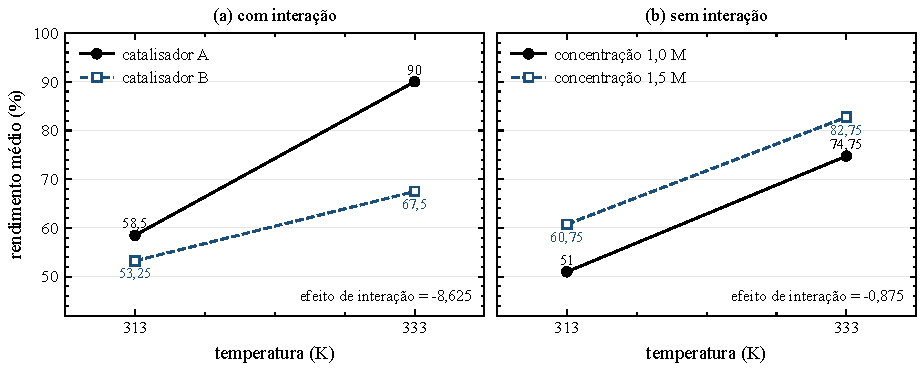
\includegraphics[width=\linewidth]{../figuras/out/c2-interacao}
  \caption{Gráfico de interação entre temperatura e catalisador (a) e entre
    temperatura e concentração (b), com as médias tomadas sobre o terceiro
    fator em cada painel. Em (a) as retas não são paralelas, sinal da
    interação $\efeito{T \cdot Cat} = -8{,}625$; em (b) as retas são
    aproximadamente paralelas, compatível com
    $\efeito{T \cdot Conc} = -0{,}875$. Dados: peixoto-2x3.}
  \label{fig:interacao}
\end{figure}

\begin{aplicacao}{Cálculo das interações temperatura$\times$catalisador e
  temperatura$\times$concentração}
  Tomando a média sobre a concentração, a resposta média em função da
  temperatura, para cada catalisador, vale
  \[
    \overline{y}_{\text{A}}(313) = 58{,}5, \quad
    \overline{y}_{\text{A}}(333) = 90{,}0, \quad
    \overline{y}_{\text{B}}(313) = 53{,}25, \quad
    \overline{y}_{\text{B}}(333) = 67{,}5 .
  \]
  O efeito da temperatura vale $90{,}0 - 58{,}5 = 31{,}5$ com catalisador A e
  $67{,}5 - 53{,}25 = 14{,}25$ com catalisador B. Pela
  Equação~\eqref{eq:interacao},
  \[
    \efeito{T \cdot Cat} = \frac{14{,}25 - 31{,}5}{2} = -8{,}625 ,
  \]
  o mesmo valor da Tabela~\ref{tab:xty}. Tomando a média sobre o catalisador,
  a resposta em função da temperatura, para cada concentração, vale
  $\overline{y}_{1{,}0}(313) = 51{,}0$, $\overline{y}_{1{,}0}(333) = 74{,}75$,
  $\overline{y}_{1{,}5}(313) = 60{,}75$ e $\overline{y}_{1{,}5}(333) = 82{,}75$,
  de modo que
  \[
    \efeito{T \cdot Conc} = \frac{(82{,}75 - 60{,}75) - (74{,}75 - 51{,}0)}{2}
                          = \frac{22{,}0 - 23{,}75}{2} = -0{,}875 ,
  \]
  um valor pequeno diante do efeito principal da temperatura, o que se
  reflete no quase paralelismo das retas do painel (b) da
  Figura~\ref{fig:interacao}.
\end{aplicacao}

\section{A matriz de contrastes e o cálculo por $\matX^{\top}\vety$}
\label{sec:contrastes}

Os cálculos das Seções~\ref{sec:efeitos-principais} e~\ref{sec:interacoes}
podem ser reunidos em um único procedimento matricial, a partir da matriz de
planejamento codificada da Tabela~\ref{tab:matriz-2x3}. Cada coluna dessa
matriz, incluindo as colunas de interação obtidas por produto de sinais,
define um contraste: a soma dos produtos entre essa coluna e o vetor de
respostas $\vety$. A definição de interação por diferença de diferenças, da
Equação~\eqref{eq:interacao}, e a definição por contraste apresentada aqui
são equivalentes: expandir os colchetes daquela equação mostra que o
resultado é exatamente a soma dos produtos entre a coluna $x_{1}x_{2}$ e o
vetor de respostas, dividida pelo mesmo divisor empregado para um efeito
principal. Sendo $N$ o número total de ensaios, a média global é o
contraste da coluna do termo independente dividido por $N$, e o efeito de
qualquer fator ou interação é o contraste da coluna correspondente dividido
por $N/2$, conforme a Equação~\eqref{eq:xty}:

\begin{equation}
  \overline{y} = \frac{\matX_{0}^{\top}\vety}{N}, \qquad
  \efeito{j} = \frac{\matX_{j}^{\top}\vety}{N/2} .
  \label{eq:xty}
\end{equation}

O divisor $N/2$, e não $N$, decorre diretamente da ortogonalidade discutida
na Seção~\ref{sec:ortogonalidade}: cada coluna de efeito tem exatamente
$N/2$ entradas iguais a $+1$ e $N/2$ entradas iguais a $-1$, de modo que o
contraste soma, com pesos unitários, $N/2$ observações de um lado contra
$N/2$ do outro.

\begin{aplicacao}{Vetor de contrastes do planejamento $2^{3}$}
  A Tabela~\ref{tab:xty} aplica a Equação~\eqref{eq:xty} às oito respostas
  médias da Tabela~\ref{tab:cubo2x3}, na ordem M, T, Cat, Conc,
  T$\cdot$Cat, T$\cdot$Conc, Cat$\cdot$Conc e T$\cdot$Cat$\cdot$Conc.

  \begin{table}[H]
    \centering
    \caption{Contrastes $\matX_{j}^{\top}\vety$ e efeitos correspondentes no
      planejamento $2^{3}$ de temperatura, catalisador e concentração.}
    \label{tab:xty}
    \begin{tabular}{l S[table-format=3.1] S[table-format=1.0]
                    S[table-format=2.4]}
      \toprule
      {Termo} & {$\matX_{j}^{\top}\vety$} & {Divisor} & {Efeito} \\
      \midrule
      M                     & 538.5  & 8 & 67.3125 \\
      T                     & 91.5   & 4 & 22.875  \\
      Cat                   & -55.5  & 4 & -13.875 \\
      Conc                  & 35.5   & 4 & 8.875   \\
      T$\cdot$Cat           & -34.5  & 4 & -8.625  \\
      T$\cdot$Conc          & -3.5   & 4 & -0.875  \\
      Cat$\cdot$Conc        & 3.5    & 4 & 0.875   \\
      T$\cdot$Cat$\cdot$Conc & 0.5   & 4 & 0.125   \\
      \bottomrule
    \end{tabular}
  \end{table}

  Os valores da última coluna reproduzem exatamente os efeitos obtidos por
  diferença de médias nas Seções~\ref{sec:efeitos-principais}
  e~\ref{sec:interacoes}, o que confirma que os dois caminhos, geométrico e
  matricial, chegam ao mesmo resultado.
\end{aplicacao}

\section{Efeito e coeficiente}
\label{sec:efeito-coeficiente}

Os mesmos dados que produzem os efeitos da Seção~\ref{sec:contrastes} também
ajustam um modelo de regressão nas variáveis codificadas, do tipo
$\hat{y} = \beta_{0} + \beta_{1}x_{1} + \beta_{2}x_{2} + \beta_{12}x_{1}x_{2}$
para o caso de dois fatores. A estimativa dos coeficientes por mínimos
quadrados é dada pela expressão já conhecida do Caderno~1,
$\hat{\vetbeta} = (\matX^{\top}\matX)^{-1}\matX^{\top}\vety$. A
ortogonalidade estabelecida na Seção~\ref{sec:ortogonalidade} torna
$\matX^{\top}\matX$ diagonal, e como cada coluna codificada em $\pm 1$ soma
$N$ quando elevada ao quadrado, todo elemento da diagonal vale $N$. A
estimativa de qualquer coeficiente se reduz, portanto, à
Equação~\eqref{eq:coeficiente}:

\begin{equation}
  \hat{\beta}_{j} = \frac{\matX_{j}^{\top}\vety}{N} .
  \label{eq:coeficiente}
\end{equation}

Comparando a Equação~\eqref{eq:coeficiente} com a
Equação~\eqref{eq:xty}, o mesmo contraste $\matX_{j}^{\top}\vety$ aparece nas
duas, dividido por $N$ para obter o coeficiente e por $N/2$ para obter o
efeito. A razão entre os dois divisores é exatamente $2$, de modo que a
Equação~\eqref{eq:efeito-e-coeficiente} vale para todo fator e toda
interação, exceto o termo independente:

\begin{equation}
  \efeito{j} = 2\hat{\beta}_{j} .
  \label{eq:efeito-e-coeficiente}
\end{equation}

A razão para o fator $2$ não é uma convenção arbitrária, mas uma consequência
direta da amplitude da escala codificada. O coeficiente $\hat{\beta}_{j}$ é a
inclinação do modelo ajustado na direção de $x_{j}$: o quanto a resposta
prevista muda por unidade de variação de $x_{j}$. Como a variável codificada
percorre toda a faixa experimental ao ir de $-1$ a $+1$, uma variação de
duas unidades, a mudança total prevista na resposta ao passar do nível baixo
para o nível alto vale $2\hat{\beta}_{j}$. Essa mudança total é, por
definição, o próprio efeito principal da Equação~\eqref{eq:efeito-principal}.
O termo independente $\beta_{0}$ escapa a essa relação porque não descreve a
variação de fator algum: ele é a própria média global, sem duplicação.

Essa distinção é a origem de um dos enganos mais comuns na leitura de saídas
de programas de análise estatística. Alguns programas, como o painel
reproduzido no conjunto aula-statistica deste caderno, apresentam colunas
separadas de efeito e de coeficiente lado a lado, o que permite conferir
diretamente que uma vale o dobro da outra. Outros programas, como o relatório
de regressão do conjunto origin-2x2, imprimem apenas a coluna de
coeficientes, e cabe ao leitor multiplicar por dois para obter o valor que
seria chamado de efeito em um relatório do primeiro tipo. Comparar, sem essa
correção, um coeficiente de um relatório com um efeito de outro superestima
ou subestima a importância prática de um fator por um fator de dois inteiro,
sem que nenhum número esteja, isoladamente, incorreto.

\begin{aplicacao}{Efeito e coeficiente no planejamento do catalisador}
  A Tabela~\ref{tab:efeito-coef} compara os efeitos e os coeficientes do
  planejamento $2^{2}$ da Tabela~\ref{tab:peixoto2x2}, ajustado com o modelo
  $\hat{y} = \beta_{0} + \beta_{1}x_{1} + \beta_{2}x_{2} + \beta_{12}x_{1}x_{2}$.

  \begin{table}[H]
    \centering
    \caption{Efeitos e coeficientes do planejamento $2^{2}$ do exemplo do
      catalisador. A razão entre as duas colunas vale exatamente $2$ para
      os três termos que descrevem fatores, e não se aplica à média.}
    \label{tab:efeito-coef}
    \begin{tabular}{l S[table-format=2.2] S[table-format=2.2]}
      \toprule
      {Termo}         & {Efeito} & {Coeficiente} \\
      \midrule
      Média           & 67.75  & 67.75 \\
      Temperatura     & 22.5   & 11.25 \\
      Catalisador     & -13.5  & -6.75 \\
      T$\cdot$Cat     & -8.5   & -4.25 \\
      \bottomrule
    \end{tabular}
  \end{table}

  Em cada uma das três linhas de fator, o efeito vale exatamente o dobro do
  coeficiente: $22{,}5 = 2 \times 11{,}25$, $-13{,}5 = 2 \times (-6{,}75)$ e
  $-8{,}5 = 2 \times (-4{,}25)$. O modelo ajustado em variáveis codificadas é
  $\hat{y} = 67{,}75 + 11{,}25\,x_{1} - 6{,}75\,x_{2} - 4{,}25\,x_{1}x_{2}$.
\end{aplicacao}

\section{O erro do efeito}
\label{sec:erro-efeito}

A estimativa de um efeito só é útil se acompanhada de uma medida de sua
incerteza. Sendo $m = 2^{k}$ o número de pontos distintos do planejamento e
$N_{j}$ o número de réplicas observadas no ponto $j$, a variância comum,
combinada entre todos os pontos, é obtida pela Equação~\eqref{eq:variancia-combinada}:

\begin{equation}
  S^{2} = \frac{\sum_{j=1}^{m} (N_{j} - 1)S_{j}^{2}}{\sum_{j=1}^{m} (N_{j} - 1)} ,
  \label{eq:variancia-combinada}
\end{equation}

com $S_{j}^{2}$ a variância amostral das réplicas no ponto $j$. A partir
dessa variância combinada, a variância de um efeito é dada pela
Equação~\eqref{eq:variancia-efeito}:

\begin{equation}
  \mathrm{Var}(\efeito{j}) = \frac{S^{2}\sum_{j=1}^{m}(1/N_{j})}{m^{2}/4} .
  \label{eq:variancia-efeito}
\end{equation}

O critério de significância compara o efeito estimado à sua incerteza por
meio de um intervalo de confiança: se
$\efeito{j} \pm t^{*}\sqrt{\mathrm{Var}(\efeito{j})}$ contém o zero, o efeito
não se distingue do ruído experimental com a confiança adotada; se não
contém, o efeito é declarado significativo. O valor crítico $t^{*}$ é o
quantil da distribuição $t$ de Student com os graus de liberdade da soma no
denominador da Equação~\eqref{eq:variancia-combinada}.

\begin{aplicacao}{Intervalo de confiança dos efeitos do catalisador}
  No planejamento $2^{2}$ da Tabela~\ref{tab:peixoto2x2}, há $m = 4$ pontos
  distintos, cada um com $N_{j} = 2$ réplicas, de modo que
  $\sum (N_{j}-1) = 4$ graus de liberdade. As variâncias de cada ponto valem
  \num{8}, \num{8}, \num{2} e \num{8}, o que dá, pela
  Equação~\eqref{eq:variancia-combinada}, $S^{2} = 26/4 = 6{,}5$. Pela
  Equação~\eqref{eq:variancia-efeito}, com $\sum(1/N_{j}) = 4 \times 0{,}5 = 2$
  e $m^{2}/4 = 16/4 = 4$,
  \[
    \mathrm{Var}(\efeito{j}) = \frac{6{,}5 \times 2}{4} = 3{,}25 ,
    \qquad \sqrt{\mathrm{Var}(\efeito{j})} = 1{,}80 .
  \]
  Com quatro graus de liberdade, o mesmo valor crítico $t^{*} = 2{,}776$ a
  95\% empregado no conjunto peixoto-saturado deste banco de números dá uma
  semi-amplitude de $2{,}776 \times 1{,}80 \approx 5{,}00$. Os três
  intervalos resultantes,
  $\efeito{T} = 22{,}5 \pm 5{,}00$, $\efeito{Cat} = -13{,}5 \pm 5{,}00$ e
  $\efeito{T \cdot Cat} = -8{,}5 \pm 5{,}00$, excluem o zero, e os três
  efeitos, inclusive a interação, são declarados significativos.
\end{aplicacao}

\section{Gráfico de Pareto dos efeitos}
\label{sec:pareto}

Quando o número de fatores cresce, cresce também o número de efeitos
principais e de interações a examinar, e uma tabela com muitas linhas de
razão $t$ é lenta de percorrer. O gráfico de Pareto dos efeitos organiza a
mesma informação da Seção~\ref{sec:erro-efeito} de forma visual, ordenando
os termos pela magnitude de seu efeito padronizado e traçando uma linha
vertical no valor crítico que separa o que é significativo do que não é.

O efeito padronizado de um termo é o módulo do efeito dividido pelo seu
erro-padrão, conforme a Equação~\eqref{eq:padronizado}:

\begin{equation}
  t_{j} = \frac{|\efeito{j}|}{\sqrt{\mathrm{Var}(\efeito{j})}} .
  \label{eq:padronizado}
\end{equation}

Essa razão é a mesma estatística $t$ empregada no teste de hipótese
$H_{0}: \efeito{j} = 0$: o intervalo de confiança da
Seção~\ref{sec:erro-efeito} exclui o zero exatamente quando $t_{j}$ excede o
valor crítico $t^{*}$ da distribuição $t$ de Student, com os mesmos graus de
liberdade do erro combinado. O gráfico de Pareto e o intervalo de confiança
são, portanto, duas leituras do mesmo teste: uma numérica, outra visual.

Os termos são ordenados por magnitude, e não pela ordem em que os fatores
foram listados, porque a pergunta que o gráfico responde é qual termo importa
mais, e a resposta é imediata quando as barras estão dispostas da maior para
a menor. Poucos termos costumam concentrar a maior parte da variação
explicada, enquanto a maioria se aproxima do ruído; ordenar por magnitude
separa esses dois grupos de forma visual, sem exigir que o leitor procure na
tabela qual valor de $p$ está abaixo do limiar adotado. A linha vertical
marca o valor crítico $t^{*}$: barras que ultrapassam a linha correspondem a
termos cujo intervalo de confiança exclui o zero, e barras que não a
ultrapassam correspondem a termos cujo intervalo contém o zero.

A Figura~\ref{fig:pareto} apresenta dois planejamentos $2^{2}$ com desfechos
opostos. O painel (a) reproduz o conjunto origin-2x2, um relatório de
regressão apenas com efeitos principais; o painel (b) reproduz o conjunto
aula-statistica, um planejamento com interação e réplicas genuínas.

\begin{figure}[H]
  \centering
  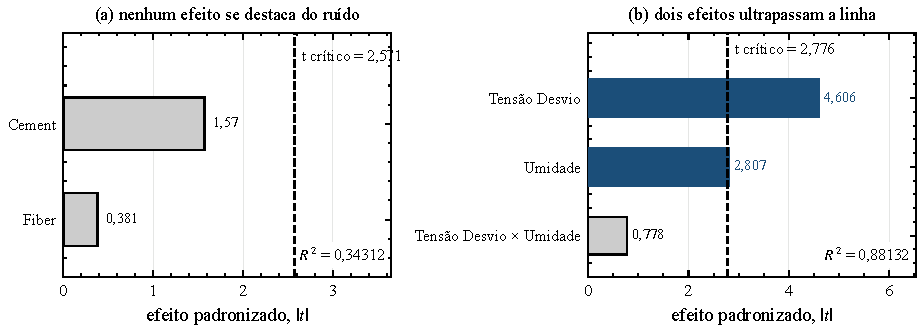
\includegraphics[width=\linewidth]{../figuras/out/c2-pareto-efeitos}
  \caption{Gráfico de Pareto dos efeitos padronizados. Em (a), nenhum dos
    dois efeitos principais ultrapassa a linha crítica de $t^{*} = 2{,}571$
    (5 graus de liberdade, 95\%), compatível com $R^{2} = 0{,}34312$. Em (b),
    dois dos três termos ultrapassam a linha crítica de $t^{*} = 2{,}776$
    (4 graus de liberdade, 95\%), compatível com $R^{2} = 0{,}88132$. Dados:
    origin-2x2 e aula-statistica.}
  \label{fig:pareto}
\end{figure}

\begin{aplicacao}{Leitura do Pareto junto da tabela ANOVA}
  No painel (a) da Figura~\ref{fig:pareto}, os efeitos padronizados valem
  $t_{\text{Fiber}} = 0{,}38139$ e $t_{\text{Cement}} = -1{,}57044$, ambos
  abaixo, em módulo, do valor crítico $t^{*} = 2{,}571$ para 5 graus de
  liberdade a 95\%. Nenhuma barra ultrapassa a linha, e a tabela ANOVA do
  mesmo relatório confirma a leitura: o teste $F$ de Fiber dá
  $p = 0{,}71858$ e o de Cement dá $p = 0{,}17711$, os dois muito acima do
  limiar usual de $0{,}05$. É o mesmo diagnóstico já sugerido pelo
  $R^{2} = 0{,}34312$ do painel, retomado com mais detalhe no Caderno~3: um
  modelo sem poder explicativo real.

  No painel (b), os efeitos padronizados valem $t = 4{,}606128$ para tensão
  desvio, $t = 2{,}807358$ para umidade e $t = 0{,}778493$ para a interação,
  contra o valor crítico $t^{*} = 2{,}776$ para 4 graus de liberdade. As duas
  primeiras barras ultrapassam a linha; a terceira, não. A tabela ANOVA
  correspondente traz $p = 0{,}009985$ para tensão desvio, $p = 0{,}048447$
  para umidade e $p = 0{,}479760$ para a interação, exatamente as duas
  primeiras abaixo de $0{,}05$ e a terceira acima. A concordância não é
  coincidência: para um termo com um grau de liberdade, o valor $F$ da ANOVA
  é o quadrado do efeito padronizado, por exemplo
  $4{,}606128^{2} = 21{,}21642$, o valor $F$ de tensão desvio impresso na
  tabela.
\end{aplicacao}

\section{Quando não há réplica}
\label{sec:sem-replica}

O critério de significância da Seção~\ref{sec:erro-efeito} depende de uma
estimativa de erro puro, e o Caderno~1 estabeleceu que réplicas genuínas são
sua única fonte. Um planejamento fatorial completo sem nenhuma réplica não
oferece essa estimativa, e nem a Equação~\eqref{eq:variancia-efeito} nem o
gráfico de Pareto da Seção~\ref{sec:pareto} podem ser construídos diretamente.

A alternativa parte de um argumento de esparsidade: na maioria dos processos,
poucos entre os $2^{k}-1$ efeitos e interações estimáveis correspondem a
fenômenos reais, e os demais se comportam como ruído. Se todos os efeitos
fossem puro ruído, cada um seria uma combinação linear das mesmas observações
e, por um argumento de tipo central, se distribuiria aproximadamente como uma
normal centrada em zero. Efeitos que se comportam como ruído, quando postos
em ordem crescente e comparados aos quantis teóricos de uma distribuição
normal padrão na mesma posição, caem próximos de uma reta; efeitos reais se
afastam dela. O procedimento consiste em ordenar os $2^{k}-1$ efeitos,
associar a cada um o quantil normal correspondente à sua posição, plotar o
par e ajustar uma reta de referência apenas pelos pontos centrais, que se
comportam como ruído, para não distorcer a reta com a presença dos efeitos
grandes.

A Figura~\ref{fig:normal-efeitos} aplica o procedimento ao planejamento
$2^{4}$ completo, sem réplica, do conjunto peixoto-2a4.

\begin{figure}[H]
  \centering
  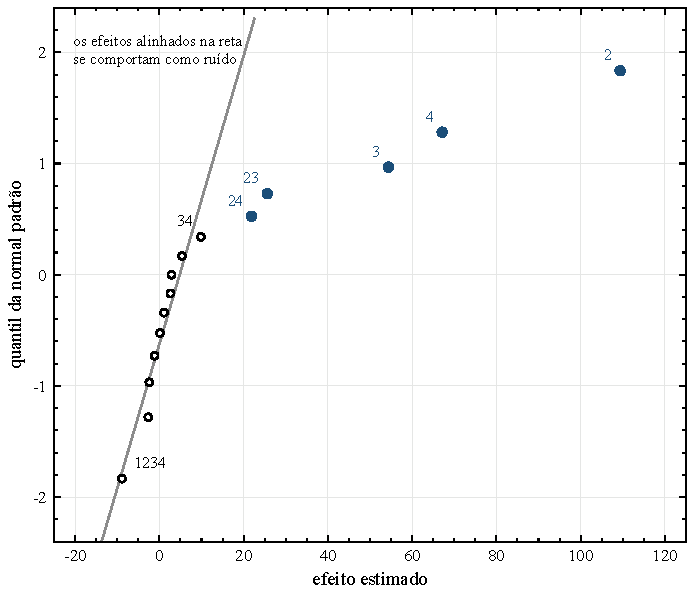
\includegraphics[width=0.75\linewidth]{../figuras/out/c2-normal-efeitos}
  \caption{Gráfico normal dos quinze efeitos do planejamento $2^{4}$ sem
    réplica. Os cinco efeitos destacados se afastam da reta ajustada pelos
    demais; os dez efeitos próximos da reta se comportam como ruído. Dados:
    peixoto-2a4.}
  \label{fig:normal-efeitos}
\end{figure}

\begin{aplicacao}{Separação de efeitos reais e ruído no planejamento $2^{4}$}
  A Tabela~\ref{tab:normal-efeitos} lista os cinco efeitos destacados na
  Figura~\ref{fig:normal-efeitos}, todos claramente afastados dos dez efeitos
  restantes, cujo módulo não ultrapassa \num{9.875}.

  \begin{table}[H]
    \centering
    \caption{Efeitos que se afastam da reta de referência no gráfico normal
      do planejamento $2^{4}$ sem réplica.}
    \label{tab:normal-efeitos}
    \begin{tabular}{l S[table-format=3.3]}
      \toprule
      {Termo} & {Efeito} \\
      \midrule
      Catalisador (2)               & 109.375 \\
      Concentração (3)              & 54.375  \\
      Temperatura (4)               & 67.125  \\
      Catalisador$\cdot$Concentração (23) & 25.625  \\
      Catalisador$\cdot$Temperatura (24)  & 21.875  \\
      \bottomrule
    \end{tabular}
  \end{table}

  Sem qualquer réplica disponível para estimar o erro puro por outra via, o
  gráfico normal permite declarar esses cinco termos como efeitos reais e
  tratar os dez restantes como ruído experimental, exatamente o papel que a
  Seção~\ref{sec:erro-efeito} atribui ao intervalo de confiança quando há
  réplica.
\end{aplicacao}

\section{Exemplo de aplicação}
\label{sec:aplicacao-final}

Esta seção percorre, do início ao fim, o planejamento $2^{3}$ de temperatura,
catalisador e concentração cujos dados alimentaram as
Seções~\ref{sec:efeitos-principais} a~\ref{sec:contrastes}, reunindo os
oito efeitos, seus erros-padrão e suas razões $t$ em uma única tabela, no
mesmo formato de saída que um programa de análise estatística produziria.

A variância combinada das oito réplicas do planejamento, com $8$ graus de
liberdade, vale $S^{2} = 5{,}1875$; o erro-padrão da média vale
$0{,}569402$ e o erro-padrão comum a todo efeito ou interação vale
$1{,}138804$. A Tabela~\ref{tab:aplicacao-2x3} reúne, para os oito termos do
modelo, o efeito, o coeficiente correspondente na escala codificada, na
razão de dois estabelecida na Seção~\ref{sec:efeito-coeficiente}, e a razão
$t$ de cada termo contra o erro-padrão do efeito.

\begin{table}[H]
  \centering
  \caption{Efeitos, coeficientes e razões $t$ do planejamento $2^{3}$ de
    temperatura, catalisador e concentração, com duas réplicas por ensaio.
    Erro-padrão do efeito de \num{1.138804}, exceto na média, cujo
    erro-padrão vale \num{0.569402}.}
  \label{tab:aplicacao-2x3}
  \begin{tabular}{l S[table-format=2.4] S[table-format=2.4]
                  S[table-format=3.2]}
    \toprule
    {Termo}                & {Efeito} & {Coeficiente} & {$t$} \\
    \midrule
    Média                  & 67.3125  & 67.3125  & 118.19 \\
    Temperatura            & 22.875   & 11.4375  & 20.09  \\
    Catalisador            & -13.875  & -6.9375  & -12.18 \\
    Concentração           & 8.875    & 4.4375   & 7.79   \\
    T$\cdot$Cat            & -8.625   & -4.3125  & -7.57  \\
    T$\cdot$Conc           & -0.875   & -0.4375  & -0.77  \\
    Cat$\cdot$Conc         & 0.875    & 0.4375   & 0.77   \\
    T$\cdot$Cat$\cdot$Conc & 0.125    & 0.0625   & 0.11   \\
    \bottomrule
  \end{tabular}
\end{table}

Contra o valor crítico $t^{*} = 2{,}306$ para $8$ graus de liberdade a 95\%,
o mesmo quantil empregado na comparação sem blocagem do conjunto armaradar
deste banco, os quatro primeiros termos de fator, temperatura, catalisador,
concentração e a interação entre temperatura e catalisador, ultrapassam a
linha crítica com folga, de $7{,}57$ a $20{,}09$ em módulo. Os três termos
restantes, as duas interações envolvendo a concentração e a interação
tripla, ficam entre $0{,}11$ e $0{,}77$, muito abaixo do valor crítico.

\begin{aplicacao}{Conclusão do planejamento $2^{3}$ do catalisador}
  A concentração do reagente tem efeito principal significativo,
  $\efeito{Conc} = 8{,}875$, com razão $t = 7{,}79$. Suas duas interações,
  porém, com a temperatura e com o catalisador, valem apenas
  $-0{,}875$ e $0{,}875$, com razões $t$ de $-0{,}77$ e $0{,}77$, muito
  aquém do valor crítico. A leitura conjunta da Tabela~\ref{tab:aplicacao-2x3}
  é que a concentração influencia o rendimento da reação, mas o faz de
  maneira essencialmente independente da temperatura e do catalisador: seu
  efeito não muda de sinal nem de magnitude relevante conforme os outros
  dois fatores variam. Na prática, isso permite que a concentração seja
  estudada em um planejamento separado, sem que a omissão de sua interação
  com os demais fatores comprometa as conclusões já obtidas para temperatura
  e catalisador.
\end{aplicacao}

O Caderno~3 retoma exatamente esse ajuste, generalizando a matriz de
planejamento em $\pm 1$ para o modelo de regressão em variáveis quaisquer, e
introduz o instrumento que falta neste caderno para julgar a qualidade do
ajuste como um todo: a decomposição da variância em $\SQR$ e $\SQr$ e o
coeficiente de determinação $\Rdois$.

\paginadireitos

\end{document}
